%! TEX root = ../main.tex
\documentclass[../main.tex]{subfiles}
\begin{document}

% ============================================================ %
% ============================================================ %
\chapter{Optimization}
% ============================================================ %
% ============================================================ %
\section{Newton's method}
The iteration is $x_{n+1} = x_n - \frac{f(x_n)}{f'(x_n)}$
\begin{figure}[!ht]
    \centering
    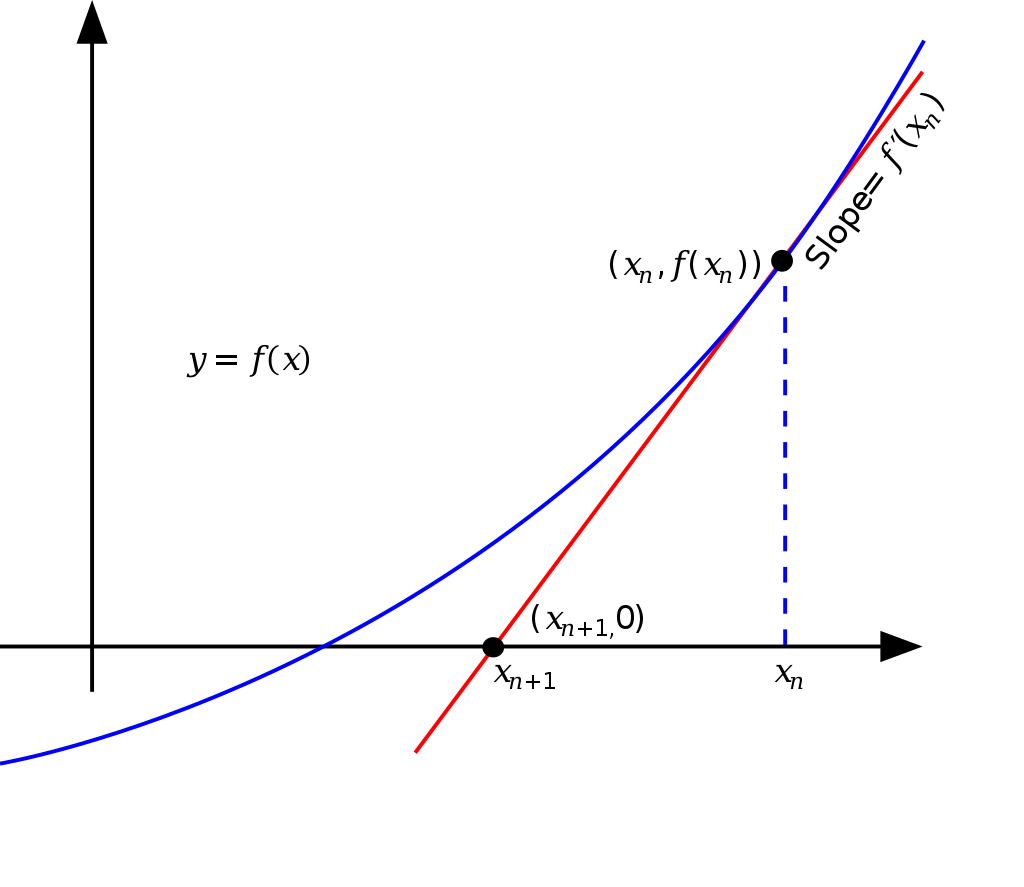
\includegraphics[height=8cm,scale=0.2]{assets/newton-method.png}
    \caption{Iteration of Newton's method}
\end{figure}
\paragraph{Convergence}
The method converges quadratically if the multiplicity of the root is 1.


\end{document}
